\chapter{Učiace sa systémy na báze odmeňovania}

V tejto kapitole budú stručne predstavené učiace sa systémy založené na odmeňovaní.
Je nevyhnutné, aspoň okrajovo spomenúť adaptívne systémy riadenia, aby bolo možné
pochopiť význam a rozdiel oproti predmetným systémom. Kapitola si kladie za cieľ
ukázať princípy, matematické detaily budú rozobraté v ďalšej kapitole.

\section{Adaptívny systém}

V teorií riadenia sa narába s pojmami spätná väzba, žiadaná hodnota,
chybová veličina, riadená sústava, regulátor a model. Obrázok \ref{img:adaptive_controll_system} zobrazuje
prepojenie základných blokov typického adaptívneho systému.


\begin{figure}[!htb]
\center
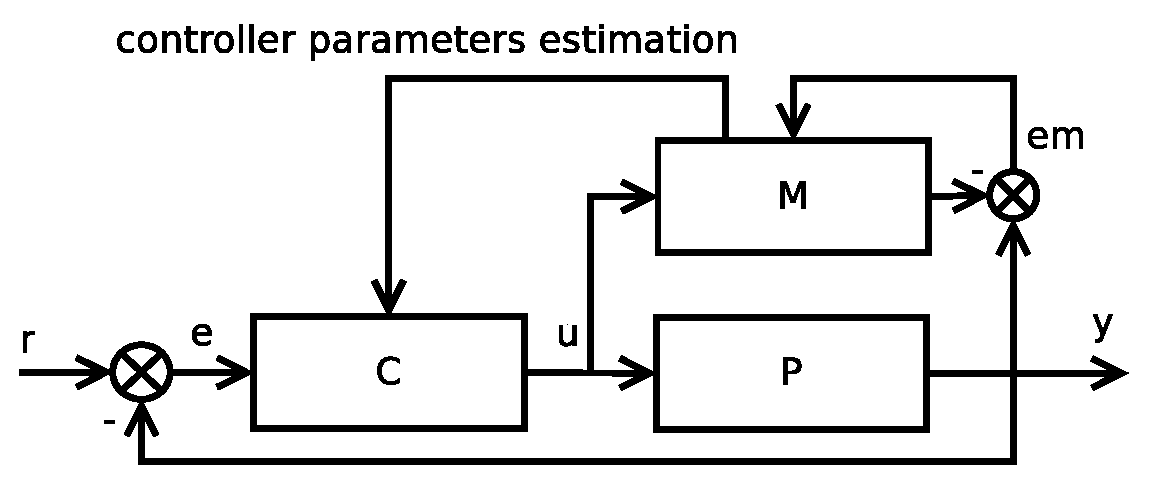
\includegraphics[scale=.6]{../diagrams/adaptive_system.eps}
\caption{Adaptívny riadiaci systém}
\label{img:adaptive_controll_system}
\end{figure}

Pre ďalšie účely sa bude hovoriť o systémoch pracujúcich v diskrétnom čase $n$ s
krokom $1$. Vstupom je žiadaná hodnota $r(n)$, výstupom je $y(n)$. Z toho nevyhnutne
vyplýva definícia chybovej veličiny ako $e(n) = r(n) - y(n)$.
Kvalitu regulátora je možné definovať rôznymi spôsobmi, najbežnejší je

\begin{equation}
K(c) = \sum\limits_{n=1}^{c}{e(n)^2}
\label{eq:controller_quality}
\end{equation}

Cieľom je minimalizovať $K(c)$. Aby existoval súčet tohto radu musí platiť $\lim_{n\to\infty}e(n)^2=0$.

Regulátor $C(n)$ je blok, tvorený obvykle diferenčnou rovnicou s volenými
parametrami do ktorého vstupuje chyba.
Veličina $u(n)$ je výstup regulátora a nazýva sa akčná veličina, predstavuje
vstup do riadenej sústavy $C(n)$. Akčná veličina ďalej vstupuje do modelu systému
ktorého parametre sa menia podľa chyby modelu $e_m(n) = y(n) - y_m(n)$, kde $y_m(n)$
je výstup modelu. Cieľom je minimalzovať $L(c) = \sum\limits_{n=1}^{c}{{e_m}(n)^2}$.
Po dosiahnutí minima sa parametre modelu rovnajú parametrom riadenej sústavy,
a je tak možné urobiť syntézu regulátora.


\section{Princípy učenia s odmneňovaním}

Pre všetky $n$ musí existovať požadovaná hodnota $r(n)$ a k nej prislúchajúca
chyba $e(n)$. Čo v prípade systémov kedy nie je pre všetky $n$ definované správanie?
Príkladom môže byť rozhodovanie robota, ktorý má splniť ciel pozostávajúci z
niekoľkých elementárnych úkonov, ale postupnosť týchto elementárnych úkonov nie je známa -
nie je teda definované $r(n)$ pre kazdé $n$.

Riešením tohto problému je zavedenie systému odmeňovania agenta (robota) \ref{img:reinforcement_learning}.

\begin{figure}[!htb]
\center
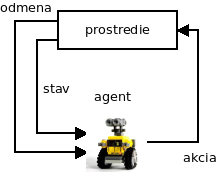
\includegraphics[scale=.8]{../diagrams/agent.png}
\caption{Učenie s odmeňovaním}
\label{img:reinforcement_learning}
\end{figure}

Táto metóda sa nazýva  {\bf reinforcement learning}. V súčastnosti predstavuje
najmocnejší nástroj strojového učenia v oblasti umelej inteligencie. Umožňuje
riešiť veľmi komplexné problémy a uplatnenie nachádza nie len v počítačových
hrách, ale napr. aj v robotike.
Jej princíp je možné zhrnúť do týchto bodov :

\begin{enumerate}
  \item Zistenie stavu
  \item Výber akcie
  \item Vykonanie akcie
  \item Prechod do ďalšieho stavu
  \item Získanie odmeny alebo trestu
  \item Učenie sa zo získanej skúsenosti
\end{enumerate}

 {\bf Zistenie stavu} je umožnené vnímaním prostredia, napr. pomocou senzorov.
V najjednoduhšom prípade si je možné ako stav predstaviť polohu. Vo
všeobecnosti, to ale nemusia byť ani priamo dáta so vstupov, ale len nejaké
príznaky - robot je na križovatke $p_0 = 0.9$, robot je v uličke $p_1 = 0.3$ .
Sada príznakov umožňuje zredukovať dimenziu stavového priestoru (tá musí
byť pre ďalej rozoberané algoritmy konečná, vyplynie to z prezentovaných rovníc).

{\bf Výber akcie} je uskutočnený na základe ohodnotení akcií získanych
v minulosti. Tieto ohodnotenia sú samozrejme závislé od stavu v ktorom sa
systém nachádza - tá ista množina akcií má iné ohodnotenie keď je robot na
križovatke a iné keď je v uličke. Vo fáze prieskumu prostredia môže agent
vyberať tie akcie ktoré boli v minulosti málo často vykonané, alebo môže vyberať náhodne.
Definovaním veľkosti zmeny ohodnotenia akcie môže uprednostniť tie akcie,
ktorých ohodnotenia vykazujú veľkú zmenu - pretože je pravdepodobné že sa
tým dostane do nepreskúmaných stavov.
Vo fáze kedy agent už nepreskúmavá prostredie, môže vyberať len najlepšie ohodnotenú akciu.
Prípadne môžu existovať v prostredí s viacerími agentami prieskumníci a vykonávatelia.
Navzájom si môžu vymieňať skúsenosti.

{\bf Vykonanie akcie} V deterministickom prostredí sa vybraná akcia vykoná vždy rovnako
(opäť však závisí na stave agenta). V nedeterministickom prostredí sa vykonanie
sa akcie riadi nejakou pravdepodobnostnou funkciou - napr. robotovi môže prešmyknúť
koleso.

{\bf Prechod do ďalšieho stavu} je obvyklým dôsledkom vykonania akcie. Samozrejme, že
v danom stave môže existovať aj taká akcia ktorá nespôsobí zmenu stavu - napr. spomínané
prešmyknutie kolesa - robot sa nepohne.

{\bf Získanie odmeny alebo trestu} po vykonaní akcie, existuje odmeňovací mechanizmus
zadaný tvorcom systému. Preto sa nedá hovoriť o umelej inteligencií - správanie
sa agenta je v deterministickom prostredí plne určené týmto mechanizmom - len nie je známe.
Obvykle platí, že kladné hodnoty dosahuje odmena, záporné trest. Nulová hodnota symbolizuje
neznalosť zadavateľa, a nevie teda určiť či dané konanie bolo dobré alebo zlé.
Nesmierne dôležitý je fakt, že pre veľkú väčšinu rozhodnutí je výsledkom odmeny práve nula.
Príkladom môže byť japonská hra Go - pre úspešné vedenie partie nestačí ohodnotiť
len aktuálny stav na gobane, je potrebné uvažovať viac ťahov dopredu - úspešnosť
ťahu sa často ukáže až po vykonaní množstva ďalších ťahov, kedy je odmena už nenulová.

Práve dominancia nulových odmien je unikátom pre reinforcement learning algoritmy.
Od zadávateľa sa vyžaduje minimum znalostí, je dokonca možné ukázať, že stačí
odmena len v cieľovom stave (i keď proces učenia bude v tomto prípade trvať veľmi dlho).


\section{Ohodnocovanie vykonaných akcií}

Odmena je získaná z prostredia po vykonaní akcie. Ohodnotenie akcie v danom stave
je tvorené predoslými skúsenosťami z vykonania predošlých akcií a získania odmien.
Podstatou učenia je teda ohodnotenie vykonaných akcií v danom stave, aby bolo
možné v každom stave rozhodnúť ktorá akcia je najlepšia - vyberá sa teda
postupnosť akcií $\pi$ pre ktorú je funkcia

\begin{equation}
\Lambda(\pi)  = \sum\limits_{n=0}^{\infty}\gamma^n R_{\pi(n)}(s(n), s(n-1))
\label{eq:q_quality}
\end{equation}

maximálna. Kde $\gamma \in \langle 0, 1 \rangle$ je koeficient zabúdania, $R_{\pi(n)}{(s(n), s(n-1)}$
je odmeňovacia funkcia po prechode zo stavu $s(n-1)$ do stavu $s(n)$ vykonaním $\pi(n)$.

Hľadanie mechanizmu nájdenia maxima $\Lambda(\pi)$ bude vysvetlené na nasledujúcich príkladoch.
\\
Pre ilustráciu bude postupnosť prechodov zapísaná priamo ako prameter funkcie $\Lambda$, napr :
$\Lambda(\{S_0, S_7, S_5\})$ predstavuje prechody z $S_0$ do $S_7$ a z $S_7$ do $S_5$.
Ďalej sa predpokladá že $\gamma = 1$.
\\
Je daný systém s troma stavmi, a dvoma prechodmi \ref{img:three_states_system}.
Pre ilustráciu je systém tak jednoduchý, že každá akcia má známu odmenu.

\begin{figure}[!htb]
\centering
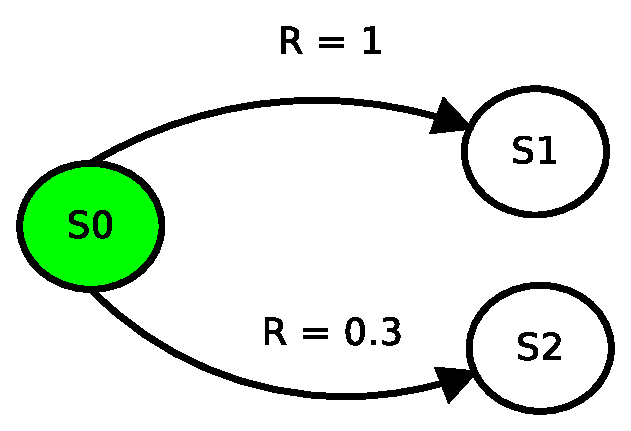
\includegraphics[scale=.6]{../diagrams/rf_two_states.eps}
\caption{Ohodnocovanie akcií v trojstavom systéme}
\label{img:three_states_system}
\end{figure}

V tomto systéme je ohodnotenie $\Lambda(S_a, S_b)$ naozaj triviálne

\begin{enumerate}
  \item $\Lambda(\{S_0, S_1\}) = 1$
  \item $\Lambda(\{S_0, S_1\}) = 0.3$
\end{enumerate}

Najlepšia cesta je potom $\{S_0, S_1\}$.

V prípade systému s viacerými stavmi \ref{img:multiple_states_system}, ale
opať známimi ohodnoteniami v každom prechode bude situácia nasledovná.

\begin{figure}[!htb]
\centering
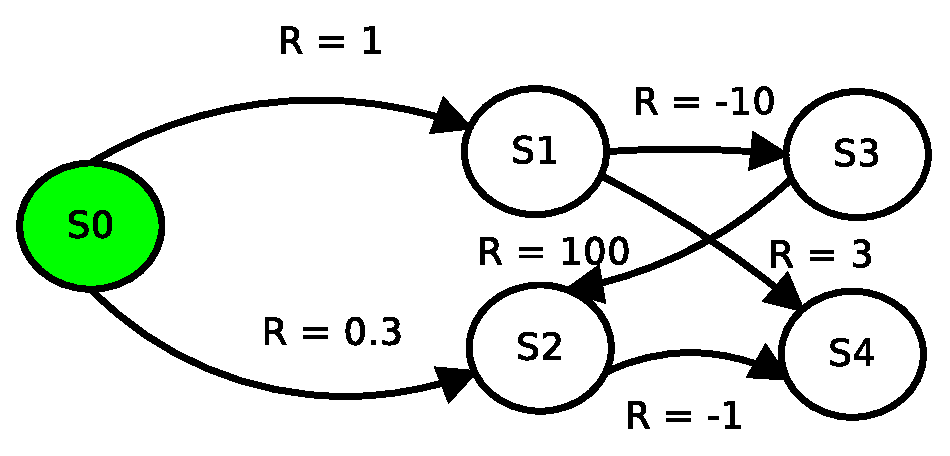
\includegraphics[scale=.6]{../diagrams/rf_more_states.eps}
\caption{Ohodnocovanie vo viacstavovom systéme}
\label{img:multiple_states_system}
\end{figure}

Ohodnotenie ciest :
\begin{enumerate}
  \item $\Lambda(\{S_0, S_1, S_3\}) = 1+(-10) = -9$
  \item $\Lambda(\{S_0, S_1, S_4\}) = 1+3 = 4$
  \item $\Lambda(\{S_0, S_2, S_4\}) = 0.3 +()-1) =-0.7$
  \item $\Lambda(\{S_0, S_1, S_3, S_2, S_4\}) = 1 +(-10) +100 + (-1) = 90$
  \item ...
\end{enumerate}

Jednoduchých ščítaním ohodnotení rôznych ciest je tak možné nájsť optimálnu
postuponosť akcií.

Ak sa v systéme nachádza cyklus \ref{img:cycle_states_system} (na obrázku
je triviálny prípad) ohodnotenie bude divergovať. Agent bude mať možnosť
vykonávať akciu ktorá neustále pripočítava kladnú odmenu, nevyhnutne tak
vyberie túto stratégiu, pretože tak získa nekonečne veľkú odmenu.

\begin{figure}[!htb]
\centering
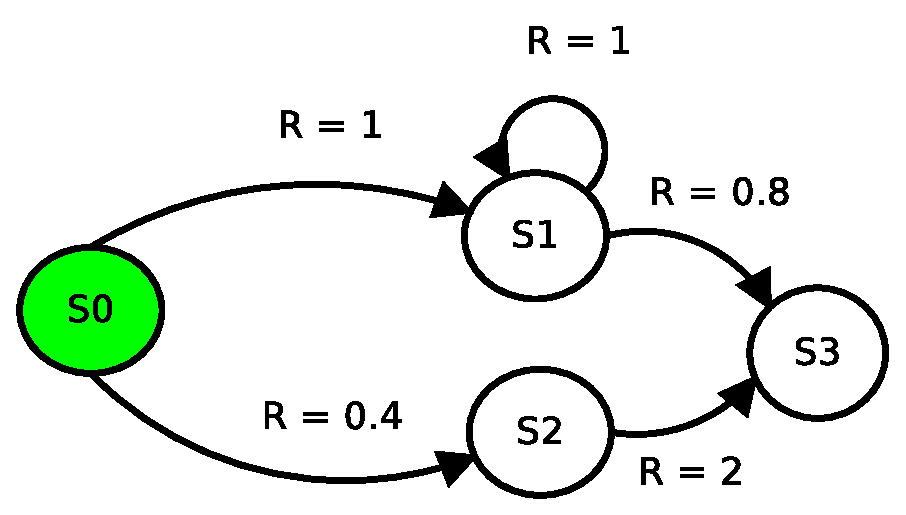
\includegraphics[scale=.6]{../diagrams/rf_cycle_states.eps}
\caption{Ohodnocovanie s cyklom}
\label{img:cycle_states_system}
\end{figure}

Ohodnotenie niektorých ciest
\begin{enumerate}
  \item $\Lambda(\{S_0, S_2, S_3\}) = 0.4+2 = 2.4$
  \item $\Lambda(\{S_0, S_1, S_3\}) = 1+1 = 2$
  \item $\Lambda(\{S_0, S_1, S_1, S_1\}) = 1+1+1 = 3$
  \item $\Lambda(\{S_0, S_1, S_1, S_1, S_1\}) = 1+1+1+1 = 4$
  \item $\Lambda(\{S_0, S_1, S_1, S_1, S_1, S_1, ...\}) = 1+1+1+1+1+...+1 = \infty$ !!!!
\end{enumerate}

Riešením je práve zavedenie faktora zabúdania $\gamma$. Ilustračne
bola zvolená $\gamma = 0.9$. Agent tak síce urobí niekoľko cyklov $S_1, S_1$,
po čase ale hodnota odmeny konverguje a minulé príspevky dávajú čoraz menší
a menší úžitok a nevyhnutne tak po niekoľkých cyklov zmení rozhodnutie a prejde
z $S_1$ do $S_3$.

Ohodnotenie niektorých ciest
\begin{enumerate}
  \item $\Lambda(\{S_0, S_2, S_3\}) = 2 + 0.9*0.4 = 2.36$
  \item $\Lambda(\{S_0, S_1, S_3\}) = 1 + 0.9*1 = 1.9$
  \item $\Lambda(\{S_0, S_1, S_1, S_1\}) = 1 + 0.9*(1 + 0.9*1) = 2.71 $
  \item $\Lambda(\{S_0, S_1, S_1, S_1, S_1\}) = 1 + 0.9*(1 + 0.9*(1 + 0.9*1)) = 3.439$
  \item $\Lambda(\{S_0, S_1, S_1, S_1, S_1, S_1, ...\}) = 10$ <-----
  \item $\Lambda(\{S_0, S_1, S_1, S_1, S_1, S_1, ..., S3\}) = 11$ <-----
\end{enumerate}

Cyklovanie v $S_1$ teda prinesie celkovú odmenu 10, ale pri prechode do $S_3$ je celková
odmena 11.

Formálny prepis uvedených úvah vedie na Q-learning algoritmus, ktorý zohľadňuje

\begin{theorem}{Bellmanov princíp optimality : }
\label{post:00}
Podstratégia optimálnej stratégie je optimálna podstratégia
\end{theorem}

\section{Jednostavový systém}

Prv než bude uvedené úplne znenie Q-learning algoritmu je vhodné rozobrať ešte
jeden príklad, a to systém s jedným stavom \ref{img:single_state_system}.
Tento problém vznikol z nasledujúcej úvahy : je daný robot ktorý má jeden senzor
vzdialenosti od cieľa (nevie teda určiť smer (napr. senzor intenzity osvetlenia) ) a možnosti pohybu o elementárny krok
vpred, vľavo, vpravo, vzad. Ako zvoliť postupnosť akcií aby robot došiel do cieľa - minimalizoval vzdialenosť?
Navyše sa predpokladá, že senzor je nekvalitný a záludný zároveň : poskytuje
informáciu len o tom či sa situácia zlepšila alebo zhoršila (oproti predošlému meraniu),
a s určitou pravdepodobnosťou generuje náhodnú hodnotu - náhodné zmení výsledok (šum).

To vedie na zostavenie odmeňovacej funkcie ako

\begin{equation}
R(n) =
\left\{
	\begin{array}{ll}
		k  & ak \ d(n) - d(n-1) < 0 \\
    -k & inak
	\end{array}
\right.
\label{eq:q_nano_r_func_simple}
\end{equation}

kde $d(n)$ je zmeraná vzdialenosť a na $d(n) - d(n-1) < 0 $ sa pozerá
ako uzavretú časť - vstupon do algoritmu teda nie je samotné $d(n)$ ale až
$R(n)$. Pre $k$ platí : $k = 1 \ ak \ rnd(0, 1) > p \ , inak \ -1$, kde $p$ je pravdepodobnosť
zmeny nameranej hodnoty $p \in \langle 0, 1 \rangle $ a $rnd(0, 1)$ generuje náhodné
číslo z intervalu $\langle 0, 1 \rangle$.

\begin{figure}[!htb]
\centering
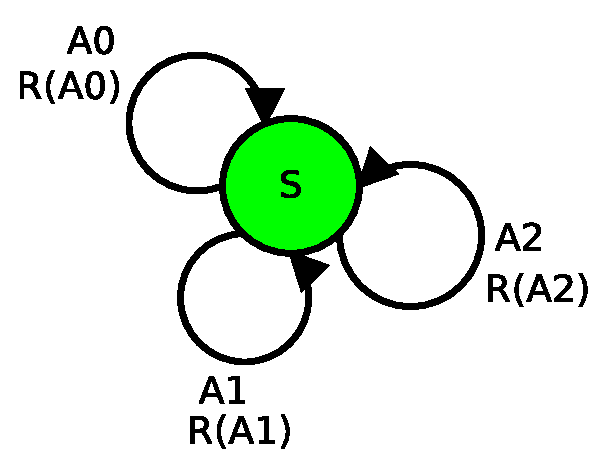
\includegraphics[scale=.6]{../diagrams/single_state.eps}
\caption{Jednostavový systém s troma akciami}
\label{img:single_state_system}
\end{figure}

Kľúčový je výber akcie $a(n)$ z konečnej množiny akcií $\mathbb{A}$,
vychádza sa z predstavy : ak má vykonaná akcia dobré ohodnotenie,
vykoná sa znova, ak má zlé ohodnotenie, vyberie sa iná, náhodná akcia.
Formálne zapísané

\begin{equation}
a(n) =
\left\{
	\begin{array}{ll}
		a(n-1)  & ak \ Q_{n-1}(a(n-1)) > 0 \\
    random() & inak
	\end{array}
\right.
\label{eq:q_nano_action_selection}
\end{equation}

Samotné $Q$ predstavujúce ohodnotenie sa potom vypočíta ako

\begin{equation}
Q_n(A(n)) = R(n) + \gamma  \max_{a'(n-1) \in \mathbb{A}} Q_{n-1}(a'(n-1))
\label{eq:nano_q_func}
\end{equation}

Algoritmus je teda veľmi jednoduchý a možno ho použit na plánovanie pohybu robota.
Robotovi tak nie vnútené správanie programátorom, ale sám sa naučí ktoré akcie
vyberať.


\subsection{Výsledky experimentu}

Overnie prebehlo s 32 virtuálnymi robotmi. Cieľom bolo naháňať pohyblivý cieľ,
ktorý sa pohyboval po kružnici. Počiatočné polohy robotov boli náhodné.
Celý experiment prebiehal v dvojrozmernom priestore obmedzenom na rozsah
polohy $\langle -1, 1 \rangle$. Metrika vzdialenosti bola Euklidovská.

Po 25000 iteráciach sa počítala priemerná chyba z 32 robotov. Vyšetrovala
sa závislosť tejto chyby od zmeny parametrov $\gamma$ a $p$ (na grafe ako gamma a noise).
Pre vybrané prípady boli exportované aj dráhy prvých 8 robotov.

Prostredie sa tak postupne mení z plne deterministického bez šumu až po hodnotu $0.4$,
čo predstavuje $40\%$ pravdepodobnosť zmeny hodnoty senzora. Graf závislosti priemernej chyby
od parametrov $\gamma$ a $p$ je na obrázku \ref{img:nano_q_summary}.

\begin{figure}[!htb]
\centering
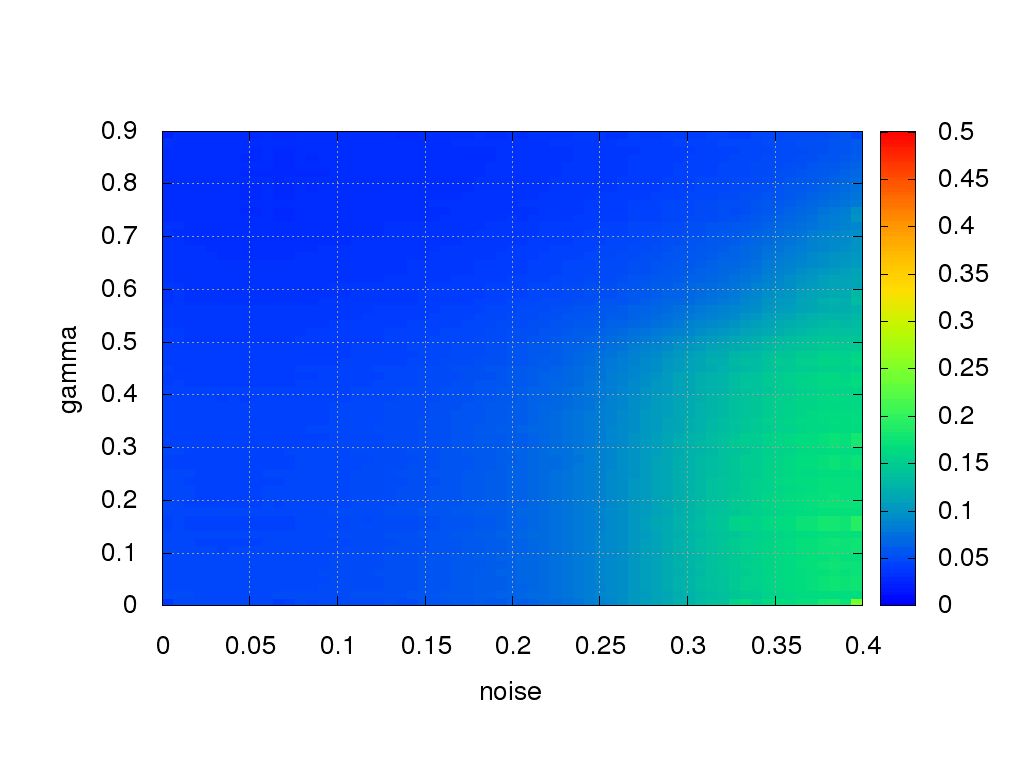
\includegraphics[scale=.4]{../../results_q_learning/nano_q_learning/summary_result_average_error_map.png}
\caption{Priemerná chyba 32 robotov po 25000 iteráciach}
\label{img:nano_q_summary}
\end{figure}

Dráhy robotov pre jednotlivé parametre :

\begin{center}
  \begin{tabular}{ | c | c || c | c |}
    \hline
    $\gamma$ & $p$ & graf dráhy & graf vývoja chyby \\ \hline
    $0.7$ & $0.0$ & \ref{img:nano_q_result_00_path} & \ref{img:nano_q_result_00_error} \\
    $0.7$ & $0.3$ & \ref{img:nano_q_result_03_path} & \ref{img:nano_q_result_03_error} \\
    $0.0$ & $0.4$ & \ref{img:nano_q_result_04_1_path} & \ref{img:nano_q_result_04_1_error} \\
    $0.7$ & $0.4$ & \ref{img:nano_q_result_04_2_path} & \ref{img:nano_q_result_04_2_error} \\
    $0.9$ & $0.4$ & \ref{img:nano_q_result_04_3_path} & \ref{img:nano_q_result_04_3_error} \\
    $0.98$ & $0.4$ & \ref{img:nano_q_result_04_4_path} & \ref{img:nano_q_result_04_4_error} \\
    \hline
  \end{tabular}
\end{center}

\begin{figure}[!htb]
\centering
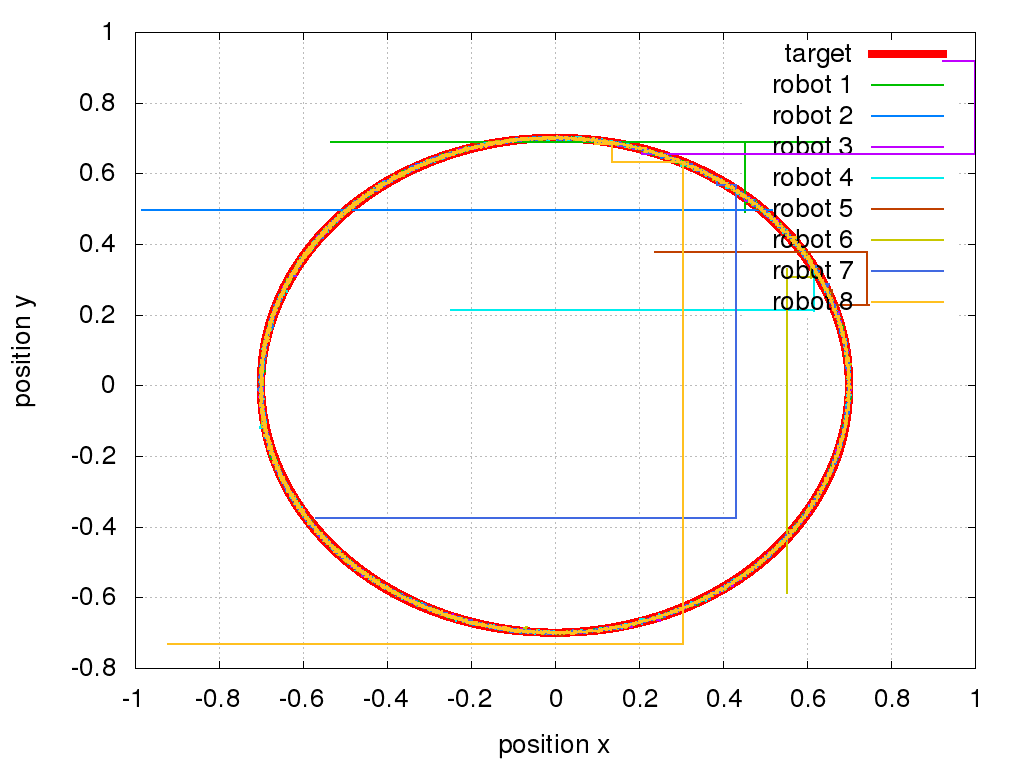
\includegraphics[scale=.4]{../../results_q_learning/nano_q_learning/result_00/robot_path.png}
\caption{Dráha robotov pre $\gamma = 0.7 p = 0.0$}
\label{img:nano_q_result_00_path}
\end{figure}

\begin{figure}[!htb]
\centering
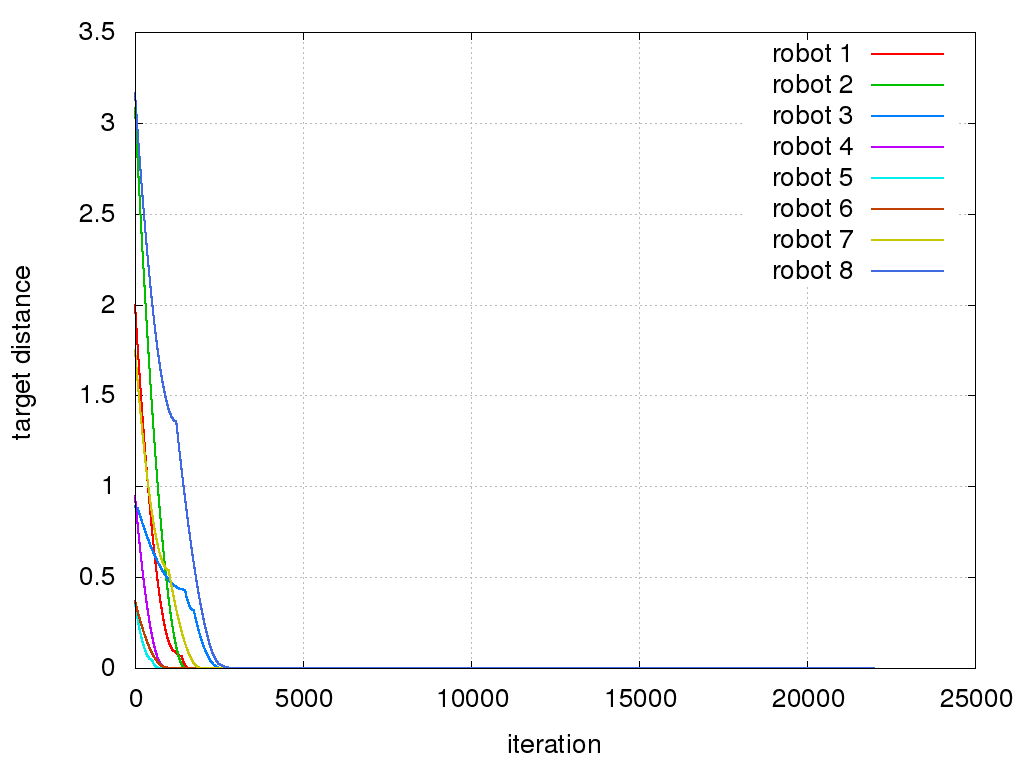
\includegraphics[scale=.4]{../../results_q_learning/nano_q_learning/result_00/robot_reward.png}
\caption{Vzdialenosť robotov od cieľa pre $\gamma = 0.7 p = 0.0$}
\label{img:nano_q_result_00_error}
\end{figure}



\begin{figure}[!htb]
\centering
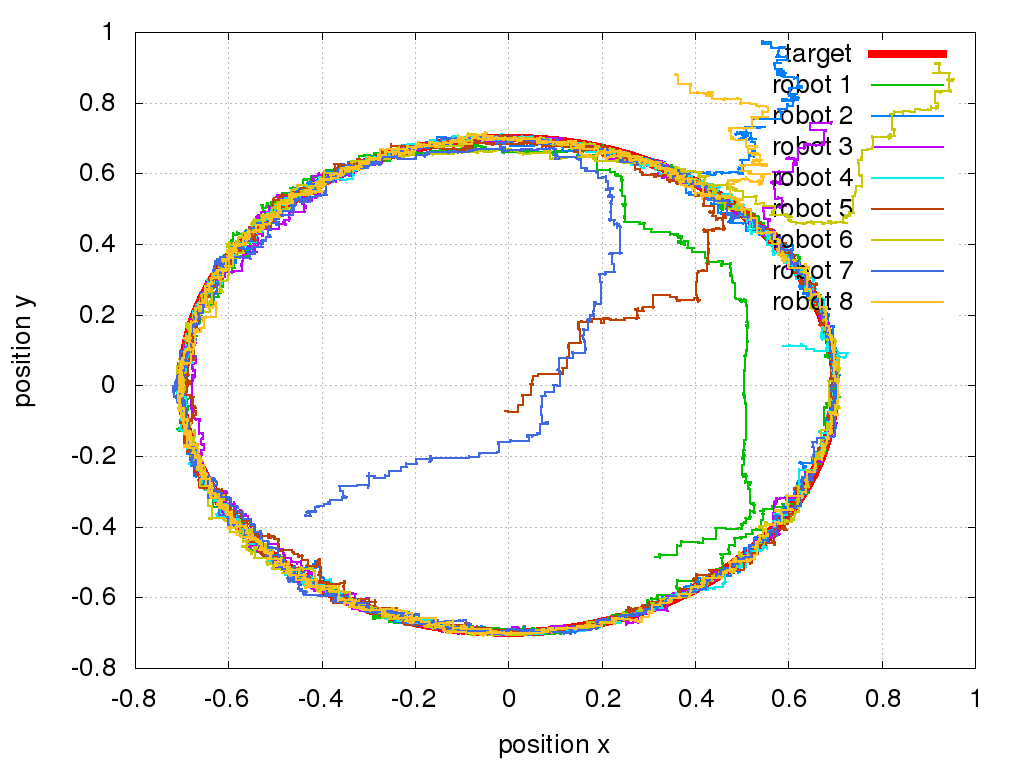
\includegraphics[scale=.4]{../../results_q_learning/nano_q_learning/result_03/robot_path.png}
\caption{Dráha robotov pre $\gamma = 0.7 p = 0.3$}
\label{img:nano_q_result_03_path}
\end{figure}

\begin{figure}[!htb]
\centering
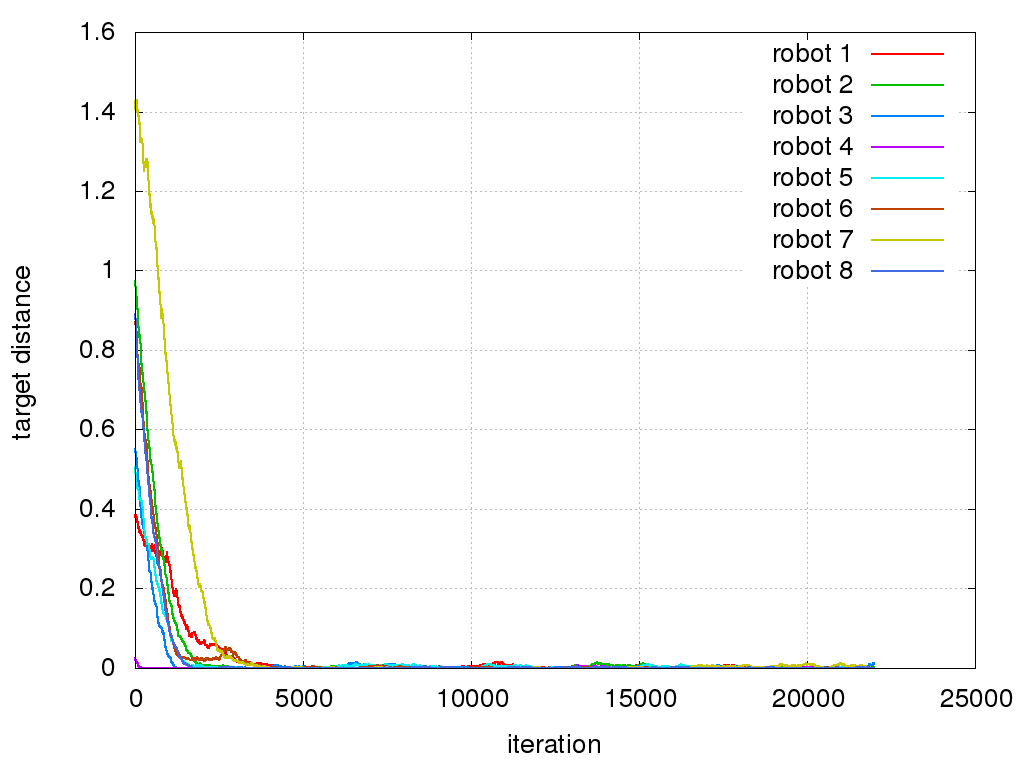
\includegraphics[scale=.4]{../../results_q_learning/nano_q_learning/result_03/robot_reward.png}
\caption{Vzdialenosť robotov od cieľa pre $\gamma = 0.7 p = 0.3$}
\label{img:nano_q_result_03_error}
\end{figure}



\begin{figure}[!htb]
\centering
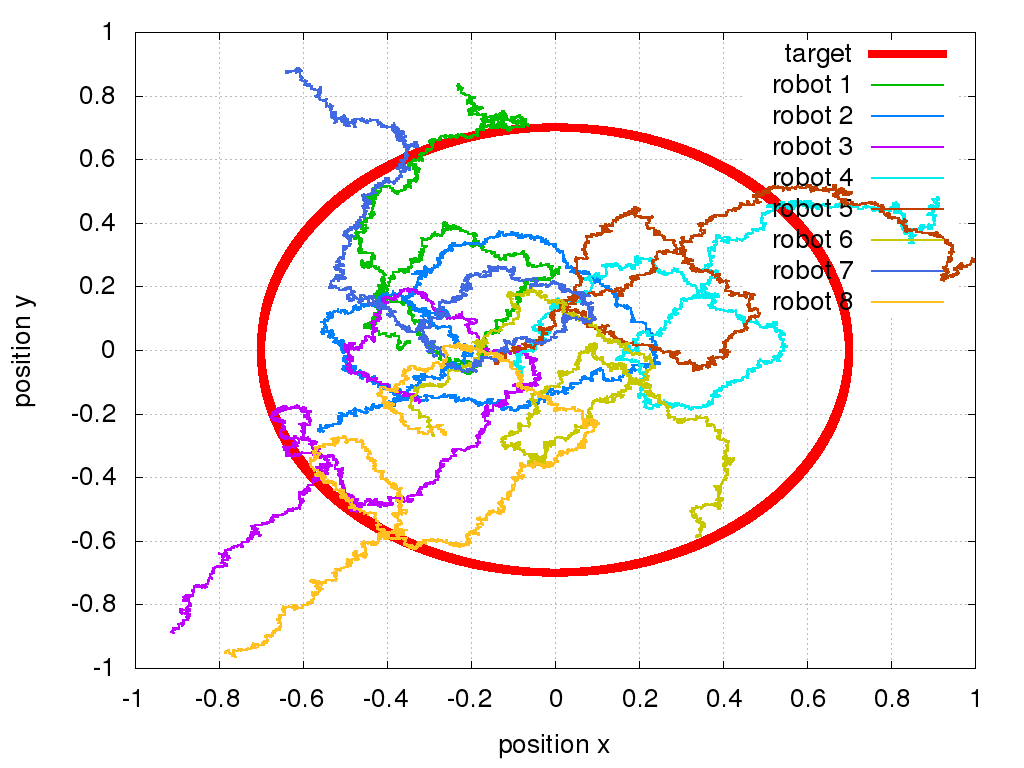
\includegraphics[scale=.4]{../../results_q_learning/nano_q_learning/result_04_01/robot_path.png}
\caption{Dráha robotov pre $\gamma = 0.0 p = 0.4$}
\label{img:nano_q_result_04_1_path}
\end{figure}

\begin{figure}[!htb]
\centering
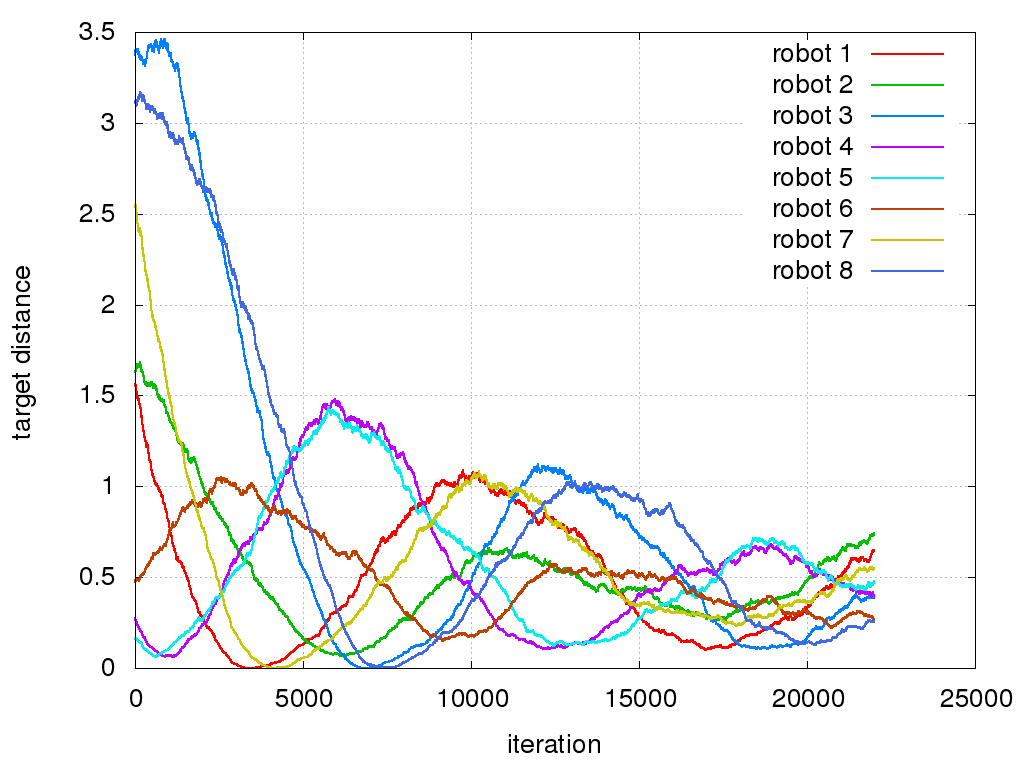
\includegraphics[scale=.4]{../../results_q_learning/nano_q_learning/result_04_01/robot_reward.png}
\caption{Vzdialenosť robotov od cieľa pre $\gamma = 0.0 p = 0.4$}
\label{img:nano_q_result_04_1_error}
\end{figure}




\begin{figure}[!htb]
\centering
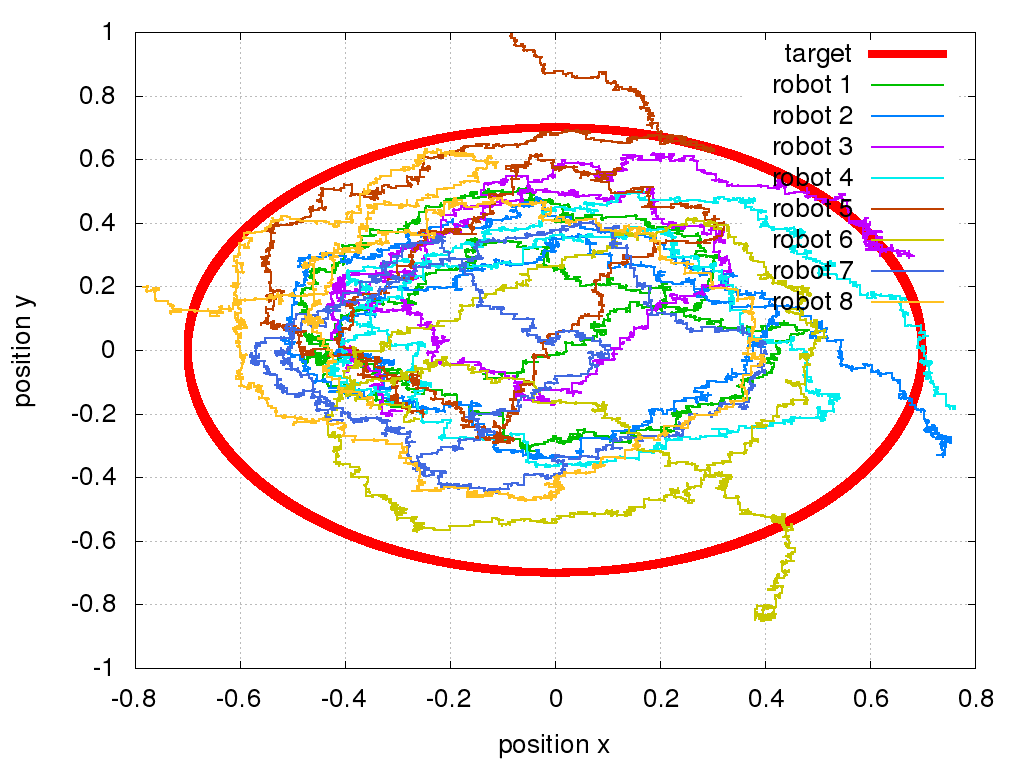
\includegraphics[scale=.4]{../../results_q_learning/nano_q_learning/result_04_02/robot_path.png}
\caption{Dráha robotov pre $\gamma = 0.7 p = 0.4$}
\label{img:nano_q_result_04_2_path}
\end{figure}

\begin{figure}[!htb]
\centering
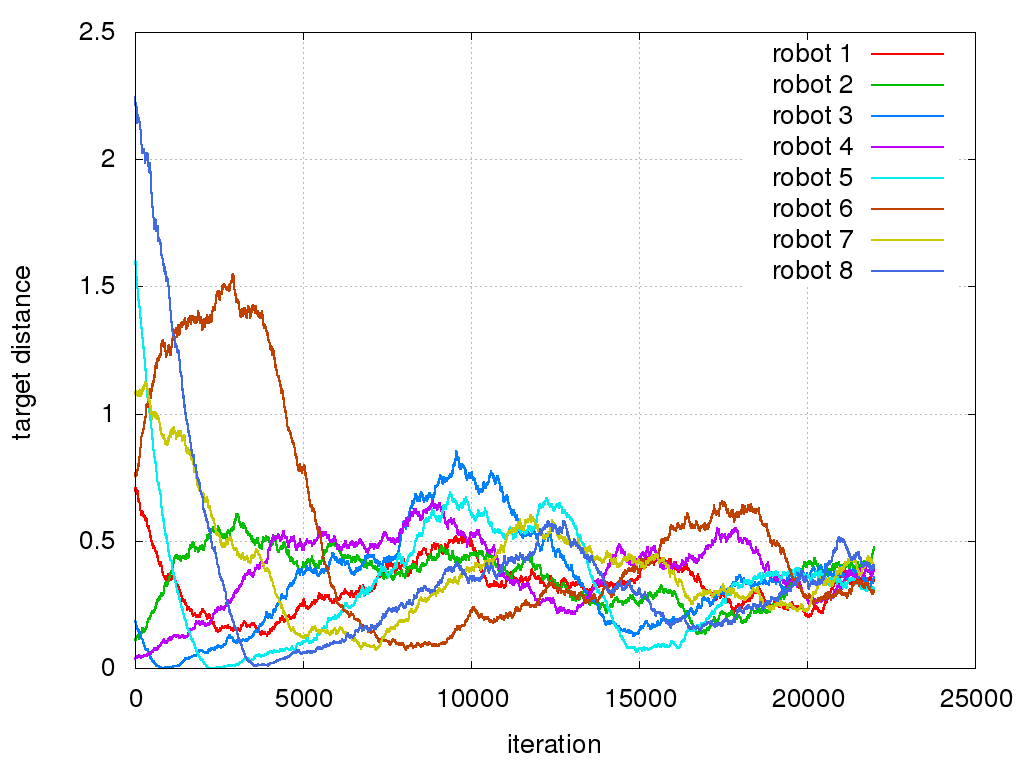
\includegraphics[scale=.4]{../../results_q_learning/nano_q_learning/result_04_02/robot_reward.png}
\caption{Vzdialenosť robotov od cieľa pre $\gamma = 0.7 p = 0.4$}
\label{img:nano_q_result_04_2_error}
\end{figure}


\begin{figure}[!htb]
\centering
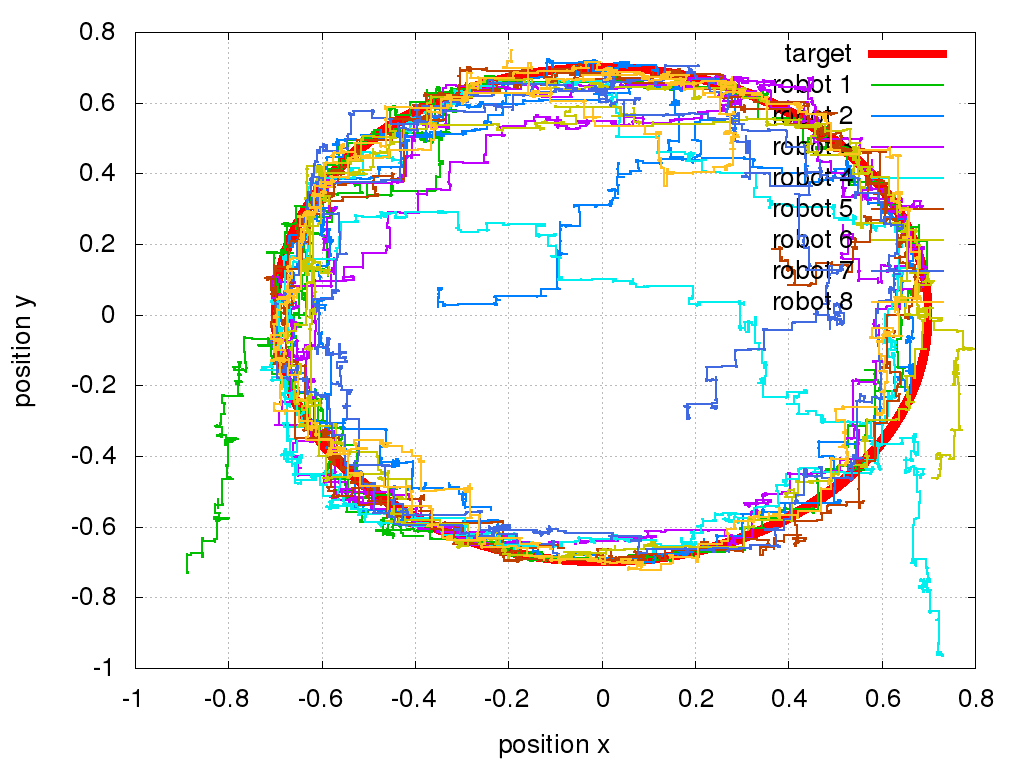
\includegraphics[scale=.4]{../../results_q_learning/nano_q_learning/result_04_03/robot_path.png}
\caption{Dráha robotov pre $\gamma = 0.9 p = 0.4$}
\label{img:nano_q_result_04_3_path}
\end{figure}

\begin{figure}[!htb]
\centering
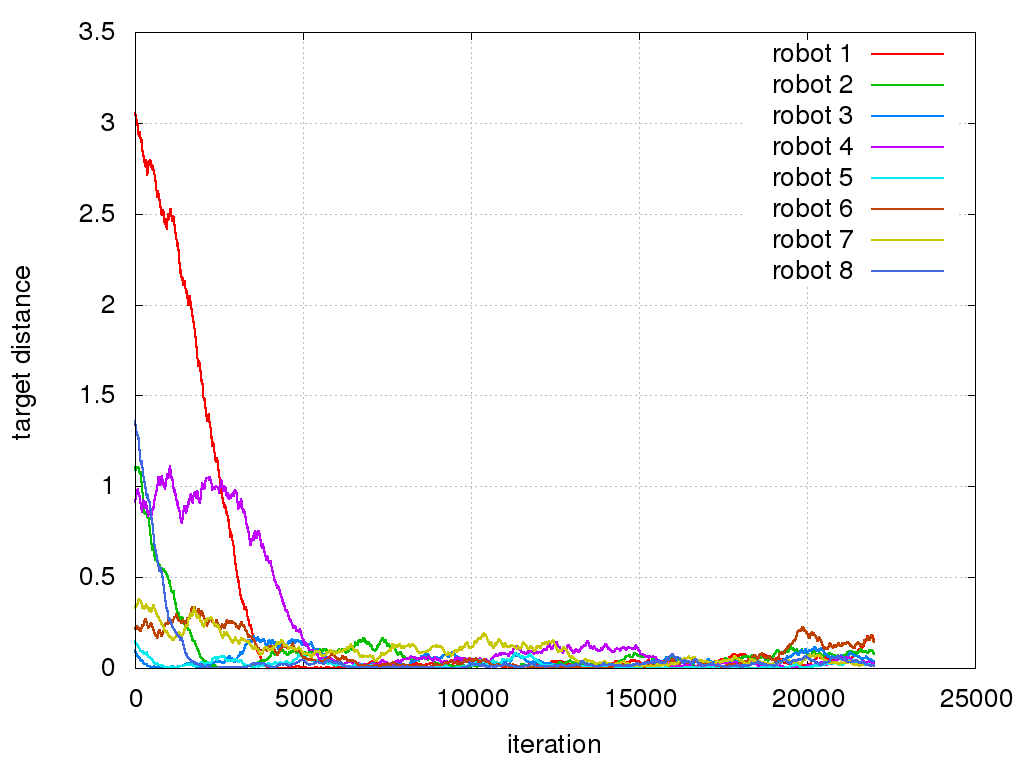
\includegraphics[scale=.4]{../../results_q_learning/nano_q_learning/result_04_03/robot_reward.png}
\caption{Vzdialenosť robotov od cieľa pre $\gamma = 0.9 p = 0.4$}
\label{img:nano_q_result_04_3_error}
\end{figure}

\begin{figure}[!htb]
\centering
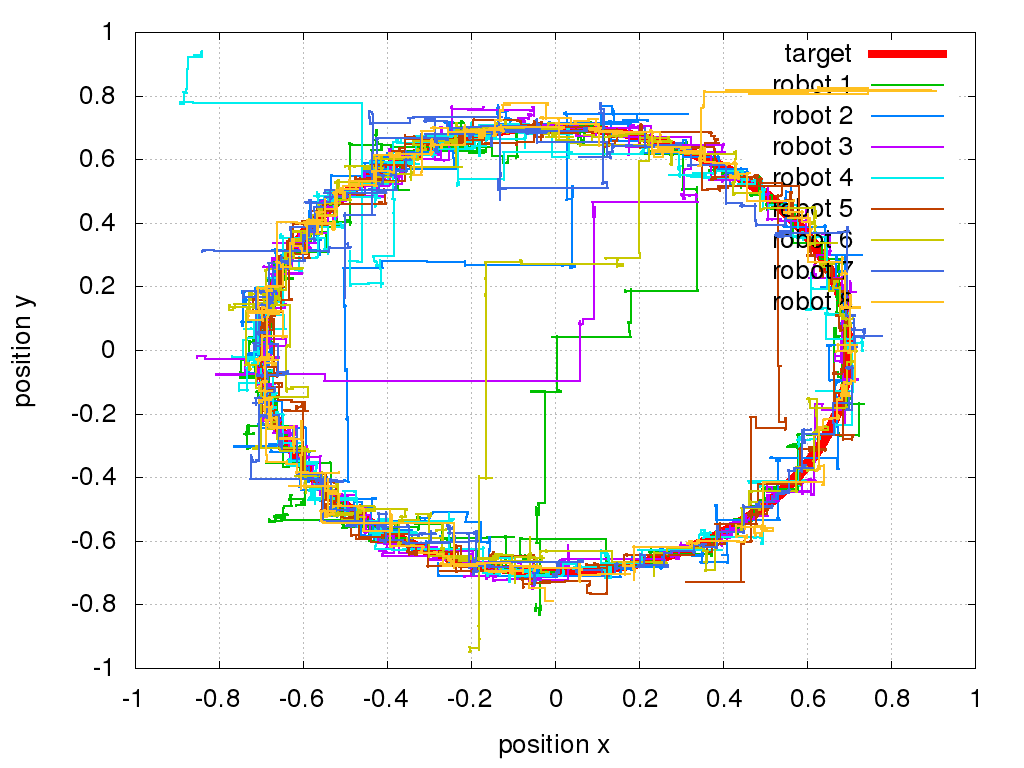
\includegraphics[scale=.4]{../../results_q_learning/nano_q_learning/result_04_04/robot_path.png}
\caption{Dráha robotov pre $\gamma = 0.98 p = 0.4$}
\label{img:nano_q_result_04_4_path}
\end{figure}

\begin{figure}[!htb]
\centering
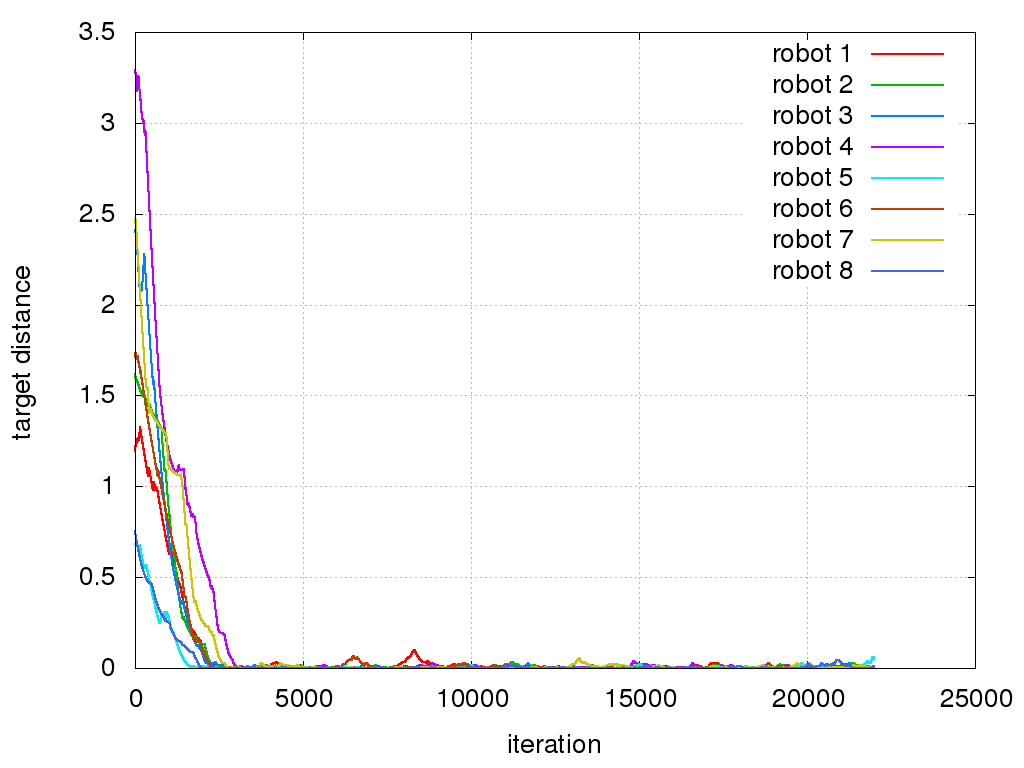
\includegraphics[scale=.4]{../../results_q_learning/nano_q_learning/result_04_04/robot_reward.png}
\caption{Vzdialenosť robotov od cieľa pre $\gamma = 0.98 p = 0.4$}
\label{img:nano_q_result_04_4_error}
\end{figure}

Z experimentov je zrejmé, že pre málo zašumené prostrednie nemá hodnota parametra
$\gamma$ veľký význam, obrázky :
\ref{img:nano_q_result_00_path}
\ref{img:nano_q_result_00_error},
\ref{img:nano_q_result_03_path}
\ref{img:nano_q_result_03_error}.

S postupným nárastom šumu však pri nevhodne zvolenej hodnote $\gamma$
roboti vykazujú veľkú chybu. Je preto tomu potrebné náležite zväčšovať
parameter $\gamma$, tento priebeh zlepšovania výsledku zvyšovaním parametra $\gamma$
je zrejmi z obrázkov :
\ref{img:nano_q_result_04_1_path}
\ref{img:nano_q_result_04_1_error},
\ref{img:nano_q_result_04_2_path}
\ref{img:nano_q_result_04_2_error},
\ref{img:nano_q_result_04_3_path}
\ref{img:nano_q_result_04_3_error},
\ref{img:nano_q_result_04_4_path}
\ref{img:nano_q_result_04_4_error}.

Algoritmus bol pomenovaný nanoQ a je pod licenciou GNU GPL dostupný na \\
https://github.com/michalnand/q\_learning/tree/master/src/nano\_q\_learning .
Je napísaný v jazyku C len s využitím pevnej rádovej čiarky. To umožňuje jeho implementáciu
aj do menej výkonných mikrokontrolérov, s jadrami napr. Cortex M0 alebo MSP430. Učenie
prebieha v reálnom čase a nevyžaduje veľký výpočtový výkon. Podobne, aj pamäťové nároky rastú
lineárne s počtom akcií. Pre veľký počet akcií je vždy možné použit aproximáciu, ktorá bude rozobratá
v neskorších častiach práce.
